\documentclass[a4paper, 10pt]{article}
\usepackage{graphicx} % Required for inserting images
\usepackage[utf8]{inputenc}
\usepackage[german]{babel}
\usepackage{geometry}
\usepackage{fancyhdr}
\usepackage{titlesec}
\usepackage{xcolor}
\usepackage{enumitem}
\usepackage{lipsum}
\usepackage{tcolorbox}
\usepackage{amsmath} % Für mathematische Formeln (optional)
\usepackage{xcolor}  % Für Farbdefinitionen
\usepackage{soul}    % Für Textmarkierung
%Seitenlayout
\geometry{top=2.5cm, left=2cm, right=2cm}

%Kopf- und Fußzeile
\pagestyle{fancy}
\fancyhf{}
\fancyhead[L]{\textbf{Operations Research 2024/25}}
\fancyhead[R]{\textbf{Lena Thuy Trang Vo}}
\fancyfoot[C]{\thepage}

%Farben 
\definecolor{lightpastelblue}{rgb}{0.80, 0.92, 0.98}
\definecolor{darkpastelblue}{rgb}{0.60, 0.80, 0.90}

% Titel-Formatierung
\titleformat{\section}{\large\color{darkpastelblue}\bfseries}{}{0em}{}[\titlerule]
\titleformat{\subsection}{\color{darkpastelblue}\bfseries}{}{0em}{}

% Definition-Box
\newtcolorbox{definitionbox}{
  colback=lightpastelblue, % Hintergrundfarbe
  colframe=darkpastelblue, % Rahmenfarbe
  fonttitle=\bfseries,
  title=Definition,
  boxrule=0.8mm, % Dicke des Rahmens
  width=\textwidth, % Breite der Box
  before=\vspace{0.5cm}, % Abstand vor der Box
  after=\vspace{0.5cm}, % Abstand nach der Box
  sharp corners=south % Scharfe Ecken unten
}


\definecolor{lightblue}{rgb}{0.80, 0.92, 0.98}
% Befehl für das Hervorheben
\sethlcolor{lightblue} % Setze die Highlight-Farbe

\begin{document}

\begin{titlepage}
    \centering
    \vspace*{3cm}
    {\Huge \textbf{Operations Research}}\\[1.5cm]
    {\large \textit{Lena Thuy Trang Vo}}\\[0.5cm]
    {\large \textit{Wintersemester 2024/25}}\\[2cm]

    \vfill
\end{titlepage}

\tableofcontents
\newpage

\section{Einführung}


\section{Kapitel 1}
\subsection{Session 1 und 2: Was sind Optimierungsmodelle und wofür kann man sie einsetzen?}
Ein Modell ist ein vereinfachtes - isomorphes oder homomorphes - Abbild eines realen Systems.
\begin{itemize}
    \item \hl{Entscheidungs- bzw. Optimierungsmodell}: formale Darstellung eines Entscheidungs- oder Planungsproblems, das in seiner einfachsten Form mindestens eine Alternativenmenge und eine diese bewertende Zielfunktion enthält
    \begin{itemize}
        \item wird entwickelt, um mit geeigneten Verfahren optimale oder suboptimale Lösungsvorschläge ermitteln zu können
    \end{itemize}

    \item \hl{Simulationsmodelle:} sind häufig sehr komplexe Optimierungsmodelle, für die keine analytischen Lösungsverfahren existieren
    \begin{itemize}
        \item dienen dem Zweck, die Konsequenzen einzelner Alternativen zu bestimmen
    \end{itemize}

    \item \hl{Beschreibungsmodelle:} beschreiben Elemente und deren Beziehungen in realen Systemen
    \begin{itemize}
        \item sie enthalten keine Hypothesen üner reale Wirkungszusammenhänge und erlauben daher keine Erklärung oder Prognose realer Vorgänge
    \end{itemize}
    \item \hl{Erklärungsmodelle:} werten empirische Gesetzesmäßigkeiten oder Hypothesen zur Erklärung von Sachverhalten aus
  
        \item \hl{Prognosemodelle:} werden in der Regel zur Gruppe der Erklärungsmodelle gezählt
        \begin{itemize}
            \item sie dienen der Vorhersage von zukünfitgen Entwicklungen
        \end{itemize}
  
    \end{itemize}
\begin{definitionbox}
    Optimierungsmodelle dienen als \textbf{Entscheidungsunterstützung} zum Finden von \textbf{Lösungen}, welche hinsichtlich eines oder mehrerer Ziele \textbf{optimiert} sind und gleichzeitig alle \hl{Restriktionen} einhalten.
\end{definitionbox}
\textbf{Bestandteile von Optimierungsmodellen}\\
\begin{figure} [h]
    \centering
    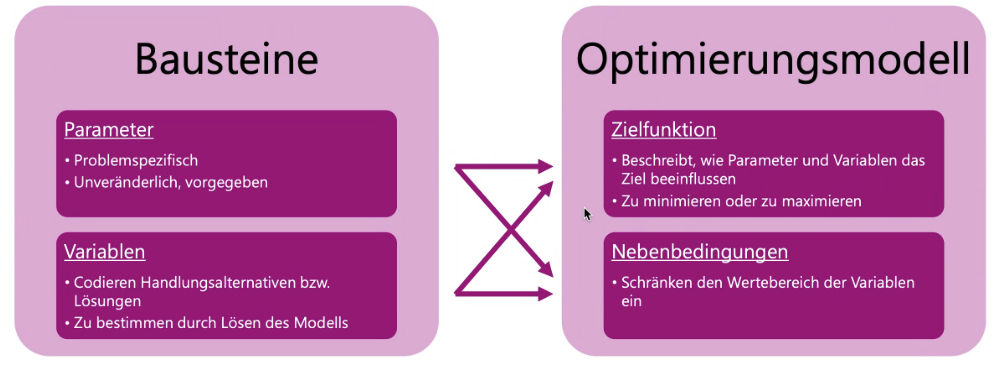
\includegraphics[width=0.7\linewidth]{/Users/lenavo/Desktop/3.Semester/Operations Research/img/bausteine.png}
    \caption{Bestandteile von Optimierungsmodellen}
    \label{fig:enter-label}
\end{figure}
\begin{itemize}
    \item Anwendungen: E-Commerce Lagerhaltung und Fahrzeugroutenplanung
\end{itemize}
\begin{definitionbox}
    Ein Optimierungsmodell, welches bezüglich der Variablen ausschließlich lineare Beziehungen enthält, nennt man \textbf{lineares Programm (LP).}
\end{definitionbox}

\subsection{Session 3: Graphisches Lösen eines Optimierungsmodells}
\begin{itemize}
    \item kann man graphisch lösen, wenn es zweidimensional ist
    \item Nebenbedingungen einzeichnen
    \item bei 2 Variablen, eine einfach gleich 0 setzen, dann die andere
\end{itemize}
\begin{definitionbox}
    Der durch die Nebenbedingungen
aufgespannte \textbf{zulässige Bereich} enthält
\textbf{alle gültigen Lösungen} des
Optimierungsproblems.
\end{definitionbox}
\begin{itemize}
    \item \hl{ISO-Linien:} Linien, die durch den Lösungsraum laufen; alle Lösungen, die auf diesen Linien liegen sind gleich gut (\textbf{selbe Lösungsqualität})
    \begin{itemize}
        \item ISO-Linien haben eine \textbf{Optimierungsrichtung}
        \item bei einer \hl{Maximierung:} möglichst weit rechts oben
        \item bei einer \hl{Minimierung:} möglichst weit links unten
    \end{itemize}
\end{itemize}

\noindent \begin{definitionbox}
    Dort, wo die \textbf{Zielfunktion} in
Optimierungsrichtung gerade noch den
\textbf{zulässigen Bereich} berührt, befindet sich
die \hl{optimale Lösung $x^*$}.
\end{definitionbox}
\textbf{Zusammenfassung des Vorgehens}\\[2mm]
\hl{Für jede Nebenbedingung:}
\begin{itemize}
    \item Überführe die Nebenbedingung in eine Geradengleichung
    \item Zeichne die Gerade in ein Koordinatensystem ein
    \item Zeichne die Wirkrichtung der Nebenbedingung ein
    \item Ergebnis: Zulässiger Bereich
\end{itemize}
 \hl{Für die Zielfunktion:}
 \begin{itemize}
     \item Setze die Zielfunktion mit einem beliebigen Wert gleich
     \item Zeichne die daraus resultierende Gerade in das Koordinatensystem ein
     \item Verschiebe die ISO-Linie parallel in Optimierungsrichtung, sodass sie gerade noch den zulässigen Bereich berührt
 \end{itemize}
 \hl{Bestimmen der optimalen Lösung:}
 \begin{itemize}
     \item Gleichsetzen der Nebenbedingungen, die sich im Berührpunkt von zulässigem Bereich und ISO-Linie schneiden
     \item Bestimmen des optimalen Zielfunktionswert durch Einsetzen der optimalen Variablenwerte
 \end{itemize}
 \subsection{Session 4: Abstrakte Optimierungsmodelle}
 \begin{definitionbox}
     Ein durch \textbf{allgemeine Parameter} formuliertes Optimierungsmodell nennt
man \textbf{abstraktes Modell}. Befüllt man das abstrakte Modell mit Werten, so
erhält man eine \textbf{konkrete Modellinstanz}.
 \end{definitionbox}
\subsection{Session 5: Summenzeichen und All-Quantoren in Optimierungsmodellen}
\begin{definitionbox}
    Mit einem \textbf{Summenzeichen} lassen sich
Terme \textbf{innerhalb von Zielfunktionen oder
Nebenbedingungen} zusammenfassen.
\end{definitionbox}
\begin{itemize}
    \item das Modell kann auch mithilfe von \hl{Indexmengen} vereinfacht werden
    \begin{itemize}
        \item Bsp. $I = \{1,2,3,\dots,100\}$
    \end{itemize}
    \item durch den \hl{Elementoperator $\in$} lässt sich dabei ausdrücken, dass eine Laufvariable Element einer Menge ist
    \begin{itemize}
        \item $i \in I$ \qquad ($i$ ist eine Element der Menge $I$)
    \end{itemize}

    \item  die Anzahl der Elemente einer Menge lässt sich durch die \hl{Kardinalität} ausdrücken
    \begin{itemize}
        \item $|I| = 100$ \qquad (Die Menge $I$ enthält 100 Elemente)
    \end{itemize}
\end{itemize}

\noindent\begin{definitionbox}
    Mit \textbf{Indexmengen} und \textbf{All-Quantoren} lassen sich
\textbf{mehrere Nebenbedingungen gleicher Struktur}
kompakt definieren.
\end{definitionbox}

\noindent\begin{definitionbox}
    Ein \textbf{abstraktes und kompaktes Optimierungsmodell} kann leichter an eine \textbf{veränderte
Problemstellung} (wie bspw. neue Maschinen oder neue Sorten) angepasst werden. Im besten
Fall ändern sich nur die \textbf{Modellbestandteile} (bspw. die Indexmengen oder Parameterwerte),
nicht jedoch die \textbf{Formulierung}.
\end{definitionbox}
\subsection{Session 6: Ganzzahligkeit}
\begin{definitionbox}
    Ein Optimierungsmodell mit ausschließlich \textbf{ganzzahligen Variablen}
heißt \textbf{IP (Integer Program)}. Ist es zusätzlich \textbf{linear}, heißt es \textbf{ILP
(Integer Linear Program)}.
\end{definitionbox}

\begin{itemize}
    \item \hl{LP:} \textbf{Jedes Wertepaar} $(x_1, x_2)$ innerhalb der Nebenbedingungen ist eine zulässige Lösung.
    \item \hl{ILP:} \textbf{Nur ganzzahlige Wertepaare $(x_1, x_2)$} innerhalb der Nebenbedinungen sind zulässige Lösungen.
\end{itemize}

\noindent\begin{definitionbox}
    Ein Optimierungsmodell, welches sowohl \textbf{ganzzahlige} als auch \textbf{kontinuierliche
Variablen}  enthält, heißt \textbf{MIP (Mixed-Integer Program)}. Ist es zusätzlich linear,
heißt es \textbf{MILP (Mixed-Integer Linear Program)}.
\end{definitionbox}
\begin{itemize}
    \item \hl{MILP:} \textbf{nur Wertepaare $( x_1, x_2)$ mit ganzzahligem $x_1$} innerhalb der Nebenbedingungen sind zulässige Lösungen.
\end{itemize}

\subsection{Session 7: Big-M Bedingungen}

\begin{definitionbox}
    Durch \textbf{binäre Variablen} lassen sich Entscheidungen mit genau \textbf{zwei Alternativen} modellieren.
\end{definitionbox}
\begin{definitionbox}
    $M$ sollte grundsätzlich \textbf{so groß wie nötig}, aber \textbf{so klein wie möglich} gewählt werden. Bei zu großen $M$ droht \textbf{numerische Instabilität}.
\end{definitionbox}

\noindent\begin{definitionbox}
    Optimierungsmodelle sind in der Regel \textbf{leichter lösbar}, wenn sie
\textbf{weniger Variablen} und \textbf{weniger Nebenbedingungen} enthalten.
\end{definitionbox}
\end{document}